\documentclass[10pt]{article}
\usepackage{icmlko}

\icmlmeta{IP 파운데이션 월드모델}{187}{달력에서만 트리를 흉내 낼 수 있었다}{노트 186이 ``달력에서 트리가 쓰는 조합을 안 봤다''를 남겼다. 도메인별 계수와 짝 곱을 명시로 넣으니 88\%가 재현된다 --- 그런데 전체 축에서는 안 된다}

\begin{document}

\twocolumn[
\icmlheader

\begin{abstract}
노트 186이 달력 열에서 트리가 $+$0.1136 을 내는데 능형이 $-$0.0244 라는
것을 보이고 ``트리가 쓰는 조합이 무엇인지 안 봤다''로 닫았다. 갈래가
둘이었다 --- 도메인마다 위상이 달라서(가)인지, 도메인 안에서 열끼리
곱해져서(나)인지. 둘을 명시로 넣어 봤다. \textbf{둘 다 필요하고 둘을
합치면 재현된다.} 풀링 선형 $-$0.024 $\to$ 짝 곱을 넣으면 $+$0.039 $\to$
도메인별 계수를 주면 $+$0.024 $\to$ \textbf{둘 다 주면 $+$0.092},
3차까지 넣으면 \textbf{$+$0.100} 이다. 트리 $+$0.114 의 \textbf{88\%}다.
\textbf{내 예측은 순서가 틀렸다} --- 도메인 이질성이 주범일 줄 알았는데
짝 곱이 더 많이 메운다($+$0.063 대 $+$0.048). \textbf{그러니 트리가
달력에서 하는 일은 신비롭지 않다} --- 도메인으로 쪼갠 뒤 열끼리 곱하는
것이고, 그것을 명시로 쓰면 해석 가능한 선형 모형이 거의 따라온다. 그다음
당연한 질문. 전체 축에서도 되나. \textbf{안 된다.} 짝 곱을 넣으면 풀링이
$+$0.0075 얻고 도메인별은 오히려 $-$0.0159 잃는다. 제일 좋은 해석 가능한
모형이 $+$0.3908 이고 트리는 $+$0.4490 이다 --- 0.058 이 안 메워진다.
\textbf{트리의 달력 우위는 설명됐고 위키 · 검색 우위는 안 됐다.} 마지막으로
이 노트가 잡은 아티팩트 하나. 처음 전체 축에서 쟀을 때 짝 곱을 넣은 판이
안 넣은 판과 \textbf{소수 넷째 자리까지 똑같이} 나왔다 --- \texttt{AXIS\_MODE}
가 ``공통''이라 전 도메인이 다 가진 축만 쓰고 도메인마다 다른 짝 곱은
조용히 버려진 것이다. \textbf{그 함정을 \texttt{F6\_directpool} 의
독스트링이 이미 적어 뒀다} --- ``차이가 정확히 $+$0.0000 으로 나온 게
단서였다.'' \textbf{여덟 번째 측정 아티팩트이고, 처음으로 내가 쓴 경고에
내가 걸렸다.}
\end{abstract}
]

\begin{figure*}[t]
\centering
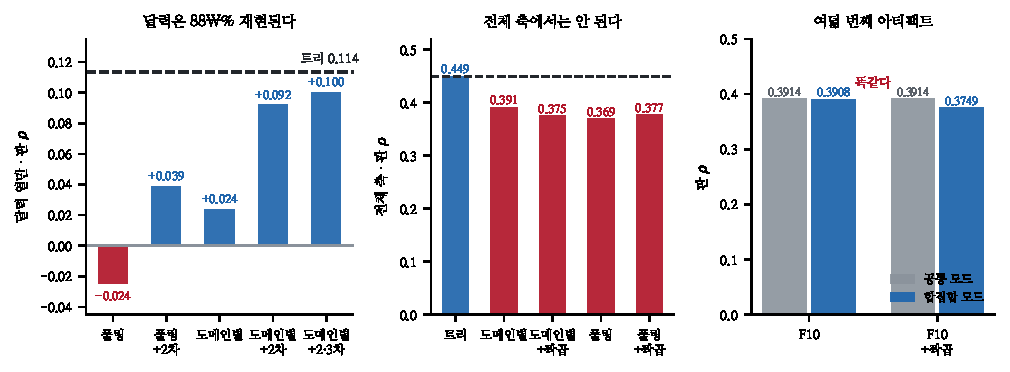
\includegraphics[width=\textwidth]{figs/mimic.pdf}
\caption{왼쪽 --- 달력은 88\% 재현된다. 가운데 --- 전체 축에서는 안 된다.
오른쪽 --- 여덟 번째 아티팩트.}
\end{figure*}

\section{달력은 재현된다}

\begin{table}[t]
\centering\tsize
\caption{달력 여섯 열만. 판 $\rho$.}
\begin{tabular}{lrr}
\toprule
& 주효과 & $+$짝 곱 \\
\midrule
풀링 선형 & \textbf{$-$.0244} & $+$.0390 \\
\textbf{도메인별 선형} & $+$.0238 & \textbf{$+$.0921} \\
도메인별 $+$ 3차까지 & & \textbf{$+$.1003} \\
\midrule
\textbf{트리} & \multicolumn{2}{c}{\textbf{$+$.1136}} \\
\bottomrule
\end{tabular}
\end{table}

\claimx{\textbf{둘을 합치면 88\%가 재현된다}($+$0.1003 대 $+$0.1136). 어느
하나만으로는 안 된다 --- 짝 곱만 $+$0.039, 도메인별만 $+$0.024.}{그러니
트리가 달력에서 하는 일은 \textbf{도메인으로 쪼갠 뒤 열끼리 곱하는
것}이다. 명시로 쓰면 해석 가능한 선형 모형이 거의 따라온다.}

\claimx{\textbf{내 예측이 순서를 틀렸다.} ``도메인 이질성이 주범''으로
$+$0.05$\sim$$+$0.09 를 적고 짝 곱은 $+$0.00$\sim$$+$0.04 로 적었는데,
실제로는 짝 곱이 더 많이 메운다($+$0.063 대 $+$0.048).}{노트 186이 달력을
``주기 열이라 위상이 도메인마다 다르다''로 읽은 것이 절반만 맞았다는
뜻이다. \textbf{``12월 그리고 주말'' 쪽이 ``도메인마다 다른 12월'' 쪽보다
크다.}}

\section{전체 축에서는 안 된다}

\begin{table}[t]
\centering\tsize
\caption{전체 열아홉 축. 합집합 모드.}
\begin{tabular}{lrr}
\toprule
& 주효과 & $+$짝 곱 \\
\midrule
풀링 선형 & .3692 & .3767 \\
도메인별 선형 & \textbf{.3908} & .3749 \\
\midrule
\textbf{트리} & \multicolumn{2}{c}{\textbf{.4490}} \\
\bottomrule
\end{tabular}
\end{table}

\claimx{\textbf{짝 곱이 거의 아무것도 안 한다.} 풀링이 $+$0.0075 얻고
도메인별은 $-$0.0159 잃는다. 제일 좋은 해석 가능한 모형과 트리 사이에
\textbf{0.058} 이 남는다.}{열 열아홉에 짝 곱 스물여덟을 더하면 마흔일곱이
되고, 유보 표본이 도메인당 수십에서 수백이라 과적합 쪽이 크다.
\textbf{달력이 여섯 열이라 됐던 것이다.}}

\claimx{\textbf{그래서 절반만 설명됐다.} 트리의 달력 우위($+$0.140)는
재현되고 위키 · 검색 우위($+$0.038)는 안 된다.}{노트 186이 세운 두
메커니즘 중 ② 비단조 · 상호작용은 달력에서 확인됐고, ① 부호 이질성은
노트 180에서 부호를 맞춰 붙여도 $+$0.0018 이었다. \textbf{위키 쪽은 아직
둘 다 아니다.}}

\section{여덟 번째 아티팩트}

\begin{table}[t]
\centering\tsize
\caption{전체 축에서 처음 잰 값.}
\begin{tabular}{lrr}
\toprule
& 공통 모드 & 합집합 모드 \\
\midrule
F10 도메인별 & .3914 & .3908 \\
F10 $+$ 짝 곱 & \textbf{.3914} & .3749 \\
\bottomrule
\end{tabular}
\end{table}

\claimx{\textbf{소수 넷째 자리까지 똑같았다.} \texttt{AXIS\_MODE} 가
``공통''이라 전 도메인이 다 가진 축만 쓰는데, 짝 곱은 도메인마다 다른 열을
곱하므로 공통이 아니다 --- \textbf{한 칸도 안 닿았다.}}{달력에서는 여섯
열이 전 도메인에 다 있어서 짝 곱 스물하나도 전부 공통이었다. 그래서 거기서는
멀쩡히 작동했고 전체 축에서만 죽었다. \textbf{같은 코드가 자료에 따라 조용히
다르게 행동한다.}}

\claimx{\textbf{그 함정을 내가 이미 적어 뒀다.} \texttt{F6\_directpool} 의
\texttt{\_feat} 독스트링에 ``처음엔 ALL5 를 그대로 돌려서, 축을 여덟 개
덧붙여도 모형에 한 칸도 안 닿았다 --- 차이가 정확히 $+$0.0000 으로 나온 게
단서였다''고 쓰여 있다.}{\textbf{여덟 번째 측정 아티팩트이고 처음으로 내가
쓴 경고에 내가 걸렸다.} 앞의 일곱은 새 실수였다 --- 순위 출력 · 라벨 적합
방향 · 복제 공선성 · 걸음 크기 · 분모 불일치 · \texttt{invalid} · 한국어
속편.}

\claimx{\textbf{그리고 단서가 같았다} --- ``정확히 같은 수''. 노트 155에서
F10 이 뒤집힌 것도, 노트 175에서 명시 축이 $+$0.0000 인 것도 같은
모양이었다.}{\textbf{규약으로 적는다: 판이 소수 넷째 자리까지 안 움직이면
바꾼 것이 모형에 안 닿은 것이다.} 개선이 없는 것과 손이 안 닿은 것은
다르다.}

\begin{table}[t]
\centering\tsize
\caption{남은 것.}
\begin{tabular}{ll}
\toprule
\textbf{위키} & 트리 우위가 아직 설명 안 됨 \\
합집합 & 트리도 합집합에서 $-$0.006 --- 왜 \\
열 수 & 마흔일곱 열은 유보 표본에 과하다 \\
\bottomrule
\end{tabular}
\end{table}

첫 줄이 남은 것 중 제일 크다. 위키 · 검색 열에서 트리가 $+$0.038 로 갈리게
이기는데(노트 186 · $t{=}2.4$), 부호를 맞춰 줘도(노트 180 · $+$0.0018)
짝 곱을 넣어도 안 따라잡힌다. \textbf{남은 후보는 결측 구조다} --- 위키
축은 덮음이 5$\sim$79\%로 도메인마다 크게 다르고, 트리는 표시자를 분기로
써서 ``관측됐나''와 ``값이 얼마나''를 곱할 수 있다. 선형은 그 곱을 못
쓴다 --- \textbf{그 곱을 명시로 넣어 보는 것이 다음이다.}

\end{document}
